% more detailed formatting: https://www.sciencemag.org/authors/instructions-preparing-initial-manuscript
% formatting: https://www.sciencemag.org/authors/science-information-authors
% submit at: https://cts.sciencemag.org/

% Reports (up to ~2500 words including references, notes and captions–corresponds to ~3 printed pages in the journal) present important new research results of broad significance. Reports should include an abstract, an introductory paragraph, up to four figures or tables, and about 30 references. Materials and Methods should be included in supplementary materials, which should also include information needed to support the paper's conclusions.

% Titles should be no more than 96 characters (including spaces).

% Short titles should be no more than 40 characters (including spaces).

% One-sentence summaries capturing the most important point should be submitted for Research Articles, Reports and Reviews. These should be a maximum of 125 characters and should complement rather than repeat the title

% Abstracts of Research Articles and Reports should explain to the general reader why the research was done, what was found and why the results are important. They should start with some brief BACKGROUND information: a sentence giving a broad introduction to the field comprehensible to the general reader, and then a sentence of more detailed background specific to your study. This should be followed by an explanation of the OBJECTIVES/METHODS and then the RESULTS. The final sentence should outline the main CONCLUSIONS of the study, in terms that will be comprehensible to all our readers. The Abstract is distinct from the main body of the text, and thus should not be the only source of background information critical to understanding the manuscript. Please do not include citations or abbreviations in the Abstract. The abstract should be 125 words or less.

% Main Text is not divided into sub-headings for Reports. Subheadings are used only in Research Articles, and Reviews.

% References and Notes are numbered in the order in which they are cited, first through the text, then through the figure and table legends and finally through Supplementary Materials.

\documentclass[11pt,letterpaper]{article}

%\usepackage{fontspec}
%\usepackage[utf8]{inputenc}
\usepackage{textcomp,marvosym}
\usepackage{amsmath,amssymb}
\usepackage[normalem]{ulem}
\usepackage[left]{lineno}
\usepackage{booktabs}
\usepackage{changepage}
\usepackage{rotating}
\usepackage{color}
\usepackage{natbib}
\usepackage{setspace}
\usepackage{array}
\usepackage{fancyhdr}
\usepackage{graphicx}
\usepackage{xspace}
\usepackage[hidelinks]{hyperref}
\urlstyle{same}
\usepackage{threeparttable}
\doublespacing

\raggedright
\textwidth = 6.5 in
\textheight = 8.25 in
\oddsidemargin = 0.0 in
\evensidemargin = 0.0 in
\topmargin = 0.0 in
\headheight = 0.0 in
\headsep = 0.5 in
\parskip = 0.1 in
\parindent = 0.2in

% Bold the 'Figure #' in the caption and separate it from the title/caption with a period
% Captions will be left justified
\usepackage[aboveskip=1pt,labelfont=bf,labelsep=period,justification=raggedright,singlelinecheck=off]{caption}

% Remove brackets from numbering in List of References
%\makeatletter
%\renewcommand{\@biblabel}[1]{\quad#1.}
%\makeatother

% Self defined commands
\newcommand{\degreesC}{\textdegree C\xspace}
\newcommand{\degrees}{\textdegree\xspace}
\newcommand{\dC}{$\delta^{13}$C\xspace}
\newcommand{\dO}{$\delta^{18}$O\xspace}
\newcommand{\SrSr}{$^{87}$Sr/$^{86}$Sr\xspace}
\newcommand{\OsOs}{$^{187}$Os/$^{188}$Os\xspace}
\newcommand{\permil}{\textperthousand\xspace}
\newcommand{\UPb}{$^{206}$Pb/$^{238}$U\xspace}
\newcommand{\pCOtwo}{\textit{p}CO$_{2}$\xspace}
\newcommand{\COtwo}{CO$_{2}$\xspace}
%

\pagestyle{myheadings}
\pagestyle{fancy}
\fancyhf{}
\lhead{Park et al., in preparation}
\rhead{\thepage}

\begin{document}

\begin{flushleft}
{\Large \textbf{Emergence of the Southeast Asian islands as a driver for Neogene cooling}}

Yuem Park\textsuperscript{1},
Pierre Maffre\textsuperscript{1},
Yves Godd\'eris\textsuperscript{3},
Francis A. Macdonald\textsuperscript{2},
Eliel A. Anttila\textsuperscript{2},
Nicholas L. Swanson-Hysell\textsuperscript{1}

\bigskip
\textsuperscript{1} Department of Earth and Planetary Science, University of California, Berkeley, CA, USA

\textsuperscript{2} Department of Earth Science, University of California, Santa Barbara, CA, USA

\textsuperscript{3} G\'eosciences Environnement Toulouse, CNRS--Universit\'e Paul Sabatier - IRD, Toulouse, France

\bigskip

\end{flushleft}

\linenumbers

\noindent
% MAXIMUM 125 CHARACTERS 
\textbf{One Sentence Summary:} The growth of tropical maritime islands led to efficient carbon consumption and drove cooling over the past 15 million years.

% MAXIMUM 125 WORDS
% NO CITATIONS OR ABBREVIATIONS
\begin{abstract}
The Southeast Asian islands bring together steep topography, a tropical climate, and mafic lithologies to efficiently weather rocks in the region and consume large amounts of \COtwo. Concurrent with global cooling since the mid-Miocene, ongoing arc-continent collision has led to a significant increase of subaerially-exposed land area in the region. Here we use geologic data to reconstruct the shorelines of the Southeast Asian islands over the past 15 million years and quantify the increase in land area. We use these paleoshorelines as boundary conditions within a coupled weathering-climate model to quantify the change in steady-state \pCOtwo associated with this emergence. We find that the modeled decrease in \pCOtwo due to these paleogeographic changes is sufficient to explain long-term climatic cooling over the Neogene.
\end{abstract}

The Southeast Asian islands (SEAI) have an out-sized contribution to modern chemical weathering fluxes. The confluence of steep topography, a warm and wet tropical climate, and the presence of mafic lithologies results in high fluxes of Ca and Mg cations and associated \COtwo consumption \cite{Gaillardet1999a}. There has been a significant increase of subaerially-exposed land area within the region since the Miocene associated with ongoing arc-continent collision between Australia and the Sunda-Banda arc system \cite{Molnar2015a, Macdonald2019a}. Concurrently, after the Miocene Climatic Optimum, a cooling trend began ca. 15~Ma and accelerated over the past 4 million years (m.y.) culminating with the onset of Northern Hemisphere glaciation \cite{Zachos2008a}. Many hypotheses have been proposed to explain this cooling trend including changes in ocean/atmosphere circulation \cite{Haug1998a, Shevenell2004a, Molnar2015a}, a decrease in volcanic outgassing \cite{Berner1983a}, or uplift in the Himalaya \cite{Raymo1992a}. Here we instead propose that SEAI emergence was itself sufficient to explain long-term climatic cooling over the Neogene.

Over geologic time-scales, \COtwo enters Earth's ocean--atmosphere system primarily via volcanism and metamorphic degassing, and leaves primarily through the chemical weathering of silicate rocks, with a smaller sink through organic carbon burial \cite{Kump1997a}. Chemical weathering delivers alkalinity and cations to the ocean which drives carbon sequestration through carbonate precipitation. Steady-state \pCOtwo is set at the \pCOtwo level at which \COtwo sinks are equal to sources. As \COtwo sinks are removed and \pCOtwo rises, temperature increases and the hydrological cycle is invigorated, causing other weathering sinks to increase until a new steady-state is achieved at higher \pCOtwo \cite{Kump1997a}. Conversely, as regions with high carbon sequestration potential emerge on Earth's surface, \pCOtwo decreases resulting in other weathering sinks to diminish leading to a new lower steady-state \pCOtwo concentration.

Topography, climate, and lithology all effect chemical weathering. High-relief regions lead to reaction-limited weathering regimes that are more sensitive to climate change \cite{Gabet2009a, West2012a}. In warm and wet regions, mineral dissolution kinetics are faster leading to enhanced chemical weathering \cite{West2012a}. Mafic rocks have higher Ca and Mg concentrations and dissolution rates than felsic rocks, and thus the potential to more efficiently sequester carbon through silicate weathering \cite{Dessert2003a}. These factors have lead to the proposal that arc-continent collisions within the tropical rain belt have been important in enhancing global weatherability, lowering atmospheric \pCOtwo, and initiating glacial climate over the past 520~m.y. \cite{Jagoutz2016a, Swanson-Hysell2017a, Macdonald2019a} and perhaps in the Neoproterozoic as well \cite{Park2019b}.

To estimate the decrease in steady-state \pCOtwo associated with the increase of subaerially-exposed land area in SEAI, we use the global spatially-resolved GEOCLIM model \cite{Godderis2017c}. GEOCLIM estimates changes in steady-state \pCOtwo associated with coupled changes in chemical weathering and climatology by linking a silicate weathering model to climate model runs at multiple \pCOtwo levels.

The silicate weathering component of GEOCLIM calculates \COtwo consumption resulting from silicate weathering for subaerially-exposed land. In previous versions of the model, silicate weathering was a function of temperature and runoff only, and all bedrock was assigned identical chemical compositions \cite{Godderis2017c}. More recent versions of GEOCLIM implement regolith development and soil shielding, which introduces a dependence on erosion (and therefore topographic slope) \cite{Maffre2018a}. While this introduction of regolith development into GEOCLIM is important for assessing the impact of tropical arc-continent collisions on \pCOtwo, the relatively high Ca+Mg concentration in arc rocks relative to other lithologies must also be considered. We therefore implement variable bedrock Ca+Mg concentration into GEOCLIM. The spatial distribution of lithologies is sourced from the Global Lithologic Map (GLiM) \cite{Hartmann2012a} and is represented by 6 categories: metamorphic, felsic, intermediate, mafic, carbonate, and siliciclastic sediment (see SI). Each land pixel is assigned these lithologic categories at a resolution of 0.1\degrees $\times$ 0.1\degrees. The Ca+Mg concentrations of felsic, intermediate, and mafic lithologies are assigned based on the mean of data compiled from EarthChem (\url{www.earthchem.org/portal}). Given that GLiM does not distinguish ultramafic lithologies, such rocks are grouped with mafic rocks. As a result, the Ca+Mg concentration is likely an underestimate in regions of obducted ophiolites, such that the estimated effect of these regions on changing steady-state \pCOtwo is conservative. The weathering of carbonate does not contribute to long-term \COtwo consumption and its Ca+Mg concentration is ignored. The Ca+Mg concentrations of metamorphic and siliciclastic sediment lithologies are more difficult to define, since their chemical composition is strongly dependent on protolith composition and, in the case of siliciclastic sediment, the degree of previous chemical depletion. We explore a range of feasible Ca+Mg concentrations for metamorphic rocks and siliciclastic sediment during calibration of the silicate weathering component.

The values of four parameters within the silicate weathering component that modify the dependence of silicate weathering on temperature, runoff, and regolith thickness are poorly constrained. Rather than prescribing values, we allow these parameters and the Ca+Mg concentration of metamorphic and siliciclastic pixels to vary within reasonable bounds (see SI). This results in 93,600 unique combinations of these six parameters. For each combination, we compute spatially-resolved long-term \COtwo consumption associated with Ca+Mg fluxes using present-day runoff, temperature, and slope. We sum computed \COtwo consumption over watersheds for which data-constrained estimates are available \cite{Gaillardet1999a, Moquet2018a}, then calculate the coefficient of determination ($r^{2}$) between computed and measured \COtwo consumption in each of these watersheds. After eliminating parameter combinations that result in low $r^{2}$, 5,381 parameter combinations remain. The resulting global \COtwo consumption of these model runs all overlap with independently-derived estimates of global \COtwo outgassing flux as they should with the long-term carbon cycle being at steady-state (see SI).

Having calibrated the silicate weathering component of GEOCLIM, we use it to estimate the decrease in steady-state \pCOtwo associated with SEAI emergence. For the climate model component, we use temperature and runoff from a subset of the GFDL CM2.0 experiments \cite{Delworth2006b} (see SI). The primary strength of these experiments for this analysis is that all non-\COtwo forcings are held constant at values representative of pre-industrial conditions, allowing the effect of changing \pCOtwo on climatology to be isolated.

To determine the position of SEAI paleoshorelines over the past 15~m.y., we use terrestrial and marine sedimentary deposits (Fig. \ref{fig:shoreline_growth}; see SI). The paleoshoreline data indicate that the Sunda-Banda Arc and New Guinea are primarily responsible for the increase in area since 15~Ma. Exhumation of the modern Sunda-Banda Arc is the result of ongoing arc-continent collision with the subducting Australian Plate \cite{Harris2006a}. Of the major islands in this arc, only Sumatra, Belitung, Bangka, Java, Bali, and Flores were subaerially exposed before 5~Ma. However, most of Sumatra and Java along with the non-volcanic islands of the Outer Banda Arc were elevated above sea level after 5~Ma \cite{Hall2013b}. In New Guinea, emergence in the Middle Miocene is associated with collision between the Melanesian Arc and Australia's distal margin \cite{Cloos2005a}, which drove exhumation of the Irian-Marum-April Ophiolite Belt. Exhumation accelerated over the past 4~m.y. in the New Guinea Central Range due to slab-breakoff and buoyant uplift, and in eastern New Guinea due to jamming of the north-dipping subduction zone \cite{Cloos2005a}. These tectonic drivers and others throughout the region lead to progressive emergence over the past 15~m.y. that accelerated following 5~Ma (Fig. \ref{fig:shoreline_growth}B). This trend mirrors broad cooling over the Neogene that resulted in the initiation of Northern Hemisphere ice sheets (Fig. \ref{fig:shoreline_growth}C). We also include changes in areas of presently-submerged continental shelves such as the Sunda Shelf that were previously exposed (see SI).

We use GEOCLIM to estimate \pCOtwo associated with the reconstructed subaerial extent of SEAI at ca. 15, 10, and 5~Ma (``paleo-SEAI'' scenarios; Fig. \ref{fig:scenario_pCO2}). Because we use a clmate model forced with modern geography, the position of the tectonic blocks remain fixed. Although there has been motion of these tectonic blocks since 15~Ma, they have remained within tropical latitudes such that this fixed scenario is a good approximation of the paleogeography (see SI). We also test an end-member scenario, in which all islands associated with arc-continent collision in the region are removed (``removed SEAI'' scenario).

Using the 5,381 unique parameter combinations, the ``paleo-SEAI'' scenarios resulted in 378--447~ppm \pCOtwo for 5~Ma, 435--532~ppm for 10~Ma, and 493--709~ppm for 15~Ma (Fig. \ref{fig:scenario_pCO2}). These results indicate a progressive decrease in \pCOtwo over the Neogene associated with the emergence of SEAI, and suggest that without this emergence, pre-industrial \pCOtwo would have been $\sim$493--709~ppm. Proxy-based estimates of the magnitude and trajectory of \pCOtwo change from the Miocene to the Pliocene are variable between techniques and associated assumptions underlying their interpretation \cite{Foster2017a}. The modeled \pCOtwo values for 15~Ma resemble the higher end of proxy-based \pCOtwo estimates for the early-mid-Miocene (see SI), indicating that the increase in subaerially-exposed land area and tectonic topography of SEAI is sufficient to explain long-term cooling of Earth's climate over the Neogene. The \pCOtwo threshold for Antarctic glaciation is estimated to be $\sim$750~ppm with that for Northern Hemisphere glaciation being significantly lower at $\sim$280~ppm \cite{DeConto2008a}. These modeled values of decreasing \pCOtwo are therefore consistent with the record of Neogene climate with Miocene ice sheets on Antarctica \cite{Sugden1995a} followed by Northern Hemisphere ice sheets developing in the Pliocene \cite{Haug2005a} as \pCOtwo subsequently decreased.

The results of our SEAI scenarios highlight the importance of the combination of topography, runoff, and lithology in setting Earth's climate state. To independently explore the effect of the modern-day surface exposure of low-relief basaltic lavas on steady-state \pCOtwo \cite{Kent2013a}, we replace mafic volcanics associated with the Deccan Traps, Ethiopian Traps, and Columbia River Basalts with the Ca+Mg concentration of bulk continental crust in GEOCLIM (Fig. \ref{fig:scenario_pCO2}). The resulting \pCOtwo is $<$500~ppm, indicating that, while the presence of mafic rocks in these igneous provinces modulates steady-state \pCOtwo as has been suggested to be important for Paleogene cooling \cite{Kent2013a}, its contribution is less than that of the wetter and higher-relief SEAI.

Other hypotheses to explain ice sheet growth over the Neogene invoke changes in ocean/atmosphere circulation including: further climatic isolation of Antarctica due to strengthening of the circumpolar current \cite{Shevenell2004a}; increased atmospheric moisture in the Northern Hemisphere due to intensified thermohaline circulation following Panama Isthmus emergence \cite{Haug1998a}; and cooling of North America resulting from a strengthened Walker Circulation associated with SEAI emergence \cite{Molnar2015a}. Such changes in ocean/atmosphere circulation are likely to modulate \pCOtwo thresholds for glacial initiation and ice sheet growth \cite{DeConto2008a}. However, the prolonged timescale of the cooling trend since 15~Ma (Fig. \ref{fig:shoreline_growth}C) is most readily attributable to decreasing \pCOtwo associated with evolving geological sources and sinks of carbon, modulated by the silicate weathering feedback \cite{Kump1997a}.

Himalayan uplift \cite{Raymo1992a} or a decrease in volcanic outgassing \cite{Berner1983a} have also been proposed as drivers for Neogene cooling. Rising marine \SrSr has been associated with increasing weathering of the high \SrSr Himalayan lithologies \cite{Raymo1992a}. This increase in \SrSr since ca. 35~Ma is followed by a decrease in slope ca. 15~Ma that has been attributed to exhumation of relatively low \SrSr and high \OsOs Lesser Himalaya lithologies \cite{Colleps2018a}, but could also be partially driven by the exhumation of mafic and organic-rich forearc sediments in SEAI during arc-continent collision. 

It continues to be argued that hypotheses that invoke enhanced weathering in regions of active uplift predict an increase in global alkalinity fluxes \cite{Si2019a}. However, total alkalinity delivery through silicate weathering needs to be nearly constant when considering the requirement of steady-state for the long-term carbon cycle. Rather, when weathering is enhanced in a region such as the emerging SEAI, the decrease in \pCOtwo results in a decrease in chemical weathering in other regions where there has not been tectonically-forced change. The same alkalinity delivery occurs more efficiently and thereby at lower \pCOtwo. Given that the weathering of carbonate is disconnected from long-term carbon-cycle mass balance, alkalinity delivery through carbonate weathering could change in an evolving climate and be observable in proxy records \cite{Si2019a}.

Changes in volcanic outgassing and paleogeography elsewhere on Earth, particularly in the Himalaya and Central America, would have effected geological carbon sources and sinks. Yet, not only does the history of SEAI emergence coincide with Neogene cooling and the onset of Northern Hemisphere glaciation, but our coupled weathering-climate model also indicates that the associated \pCOtwo change is sufficient to explain the magnitude of cooling. These results highlight that the Earth's climate state is particularly sensitive to changes in tropical paleogeography.

%%TC:ignore
\section*{ACKNOWLEDGEMENTS \label{sec:ACKNOWLEDGEMENTS}}

Collaborative research between NLS-H and YG was initially supported by a grant from the France-Berkeley Fund. FAM and NLS-H gratefully acknowledge support through NSF FRES grants \#1926001 and \#1925990. We thank Alec Brenner, Sam Lo Bianco, Mariana Lin, and Judy Pu for their data compilation contributions to the paleoshoreline reconstructions. The GEOCLIM code associated with this study is openly available: \url{https://github.com/piermafrost/GEOCLIM-dynsoil-steady-state}
%%TC:endignore

\clearpage
\newpage

\section*{FIGURES}

% 70 words
\begin{figure}[h!]
    \centering
    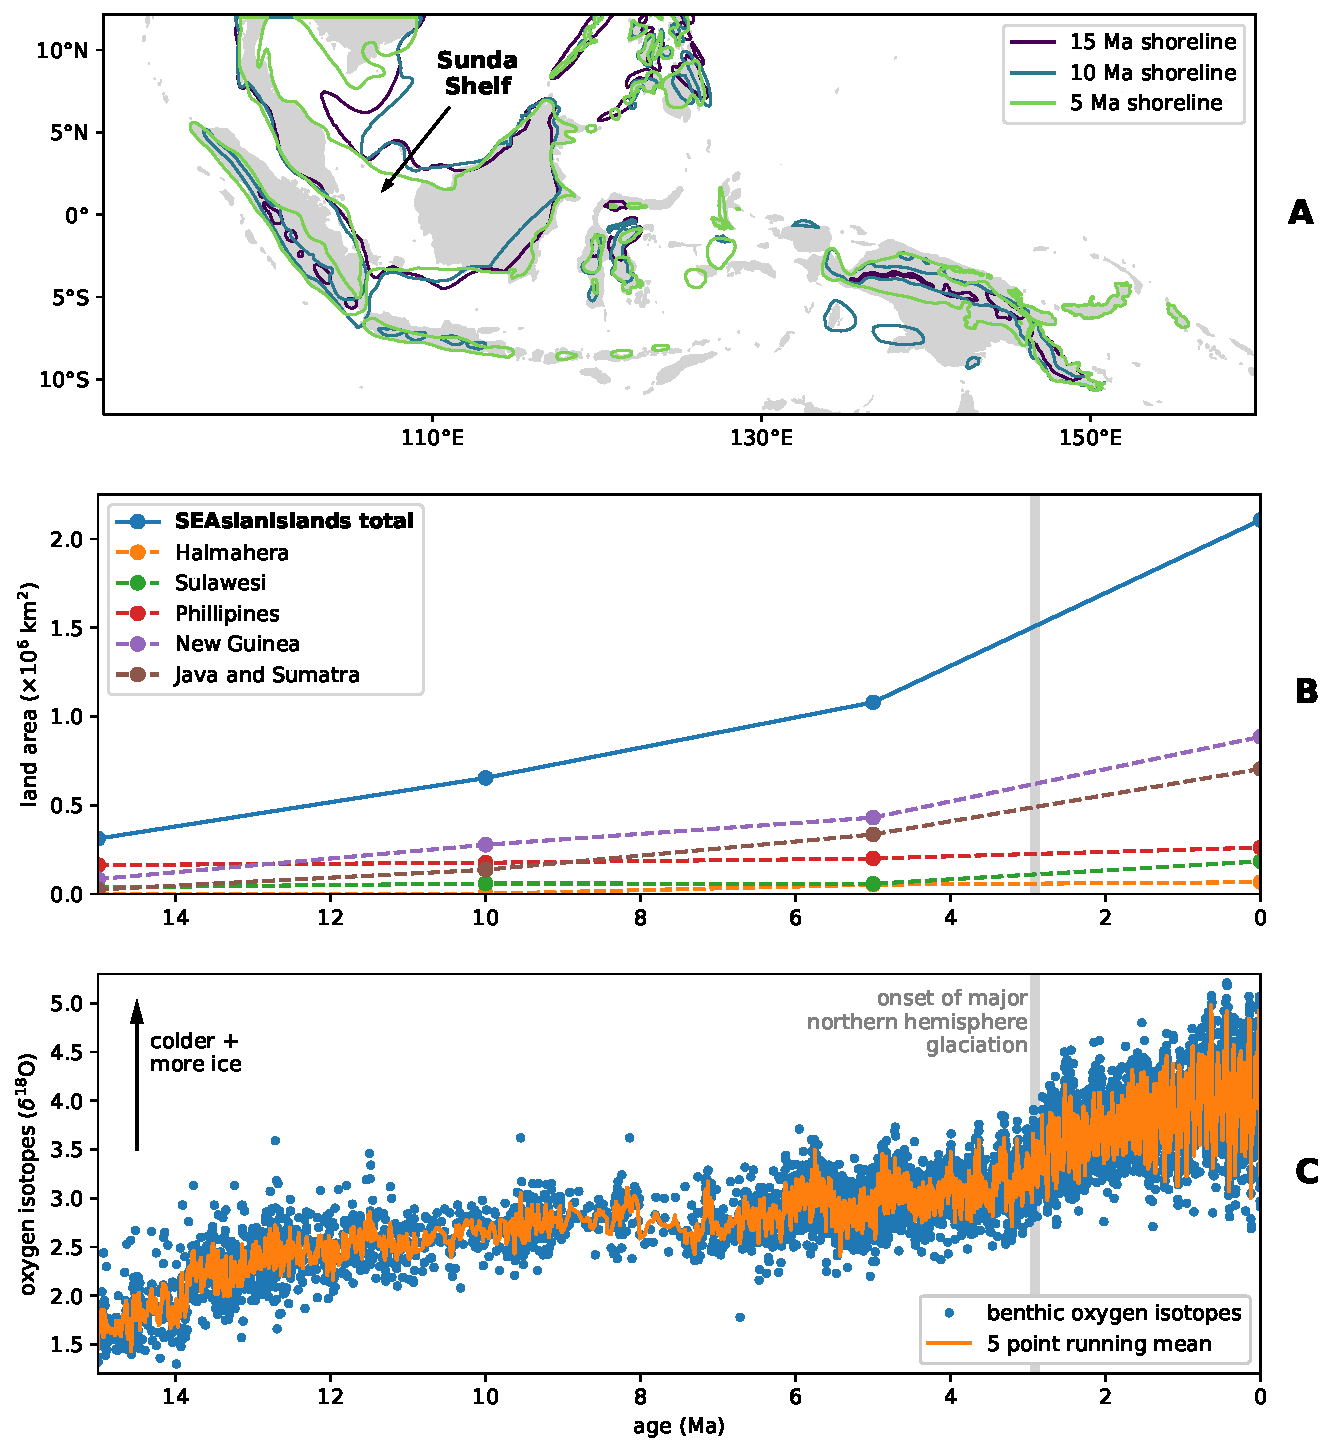
\includegraphics[width=0.9\textwidth]{Figures/shoreline_growth.pdf}
    \caption{The emergence of the Southeast Asian islands (also referred to as the Maritime Continent in climate science literature) from the mid-Miocene to present. Past shorelines are shown in A with associated land area summarized in B. A significant increase in area over the past 5 million years is coincident with cooling and the onset of Northern Hemisphere glaciation as reflected in the benthic oxygen isotope record \cite{Zachos2008a} shown in C.}
    \label{fig:shoreline_growth}
\end{figure}

% 100 words
\begin{figure}[h!]
    \centering
    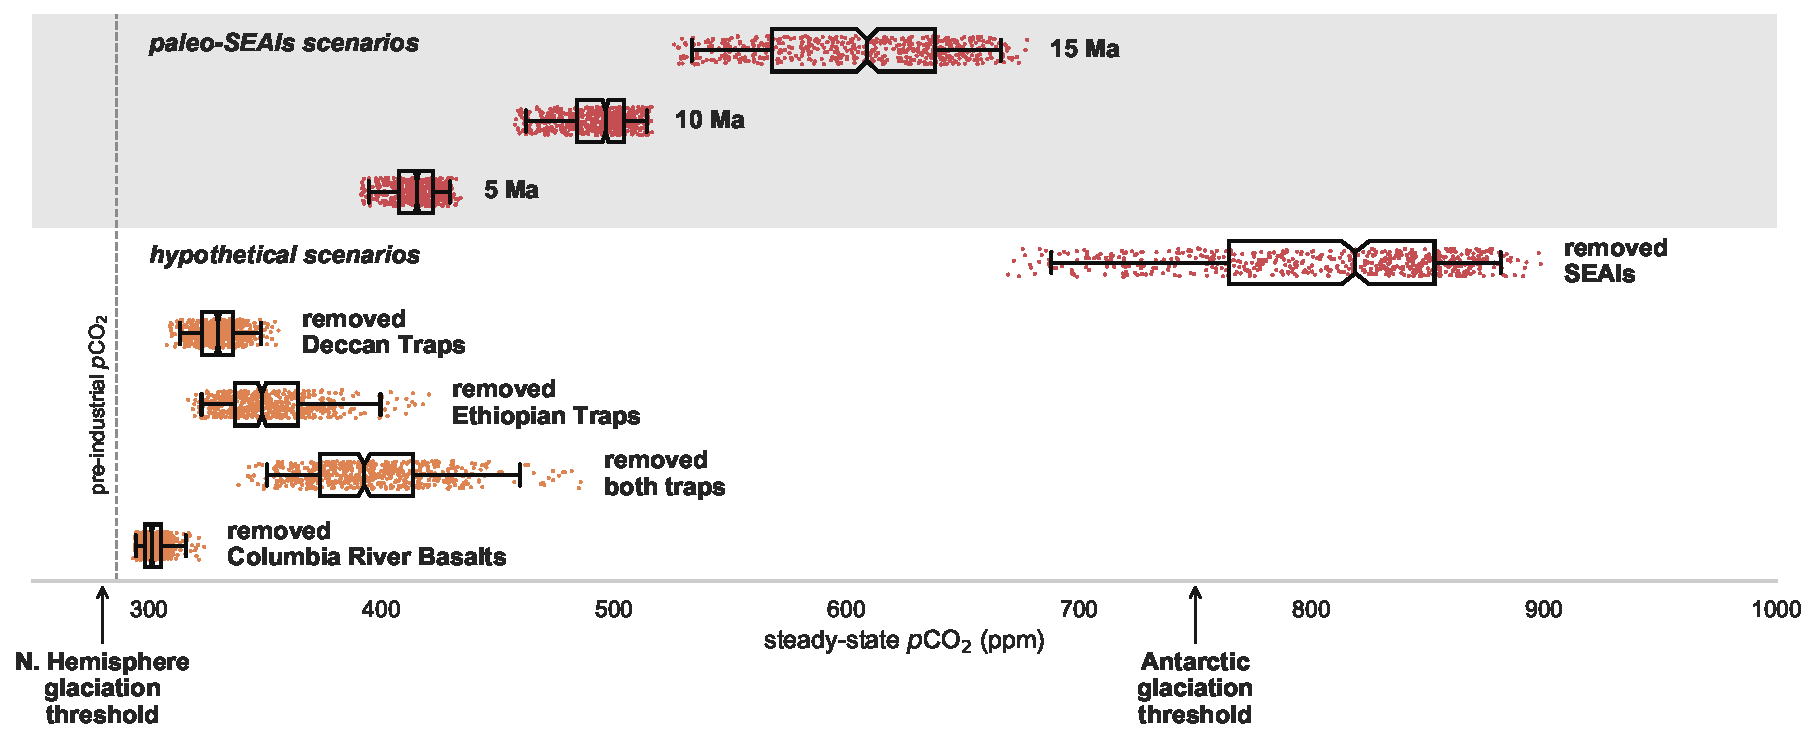
\includegraphics[width=1\textwidth]{Figures/scenario_pCO2.pdf}
    \caption{Steady-state \pCOtwo estimates from GEOCLIM for the various scenarios discussed in the text. For each of the seven scenarios, each point represents an estimate from one of the 5,381 unique parameter combinations that resulted in reasonable total global \COtwo consumption and most closely matched estimates of present-day \COtwo consumption in 80 watersheds around the world (see SI). The box encloses the middle 50\% of the \pCOtwo estimates (i.e. the interquartile range), and the notch represents the median with its 95\% confidence interval. The whiskers extend to the 2.5 and 97.5 percentile values. Glaciation thresholds \cite{DeConto2008a} are shown on the x-axis.}
    \label{fig:scenario_pCO2}
\end{figure}

\clearpage
\newpage
\footnotesize

\singlespacing

\bibliographystyle{nature}
\bibliography{References}

\end{document}